\begin{example}[twoRounds]
    \label{ex:twoRounds}
    In this example program $\kw{towRounds(k)}$, the analyst asks in total $k+1$ queries to the mechanism in two phases.
    In the first phase, the analyst asks $k$ queries and stores the answers that are provided by the mechanism. 
    In the second phase, the analyst constructs a new query based on the results of the previous $k$ queries and sends this query to the mechanism. More specifically, we assume that, in this example, the domain $\dbdom$ 
    contains at least $k$ numeric attributes, which we index just by natural numbers. 
    The queries inside the while loop correspond to the first phase and compute an approximation of 
    the product of the empirical mean of the first $k$ attributes. 
    The query outside the loop corresponds to the second phase and computes an approximation of the empirical mean where each record is weighted by the sum of the empirical mean of the first $k$ attributes.
    %
    % Queries are of the form $q(e)$ where $e$ is an expression with a special variable $\chi$ representing a possible row. Mainly $e$ represents a function from $X$ to some domain $U$, for example $U$ could be $[-1,1]$ or $[0,1]$. This function characterizes the linear query we are interested in running. As an example, $x \leftarrow q(\chi[2])$ computes an approximation, according to the used mechanism, of the empirical mean of the second attribute, identified by $\chi[2]$. Notice that we don't materialize the mechanism but we assume that it is implicitly run when we execute the query. 
    % \jl{We use $\chi$ to abstract a possible row in the database and }
    % queries are of the form $\query(\qexpr)$, where $\qexpr$ is a special expression 
    %
    {Since statistical query computes the empirical mean of a function on rows, we use $\chi$ to abstract a possible row in the database and }
    queries are of the form $\query(\qexpr)$, where $\qexpr$ is a special expression 
    (as in our syntax in Section~\ref{sec:language})
    {
    % from $X$ to some domain $U$, 
    % for example $U$ 
      We use $U$ to denote the co-domain of queries, and it could be $[-1,1]$, $[0,1]$ or $[-R,+R]$, for some $R$ we consider.
      This function characterizes the linear query we are interested in running. 
      As an example, $x \leftarrow \query(\chi[j] \cdot \chi[k])$ computes an approximation, according to the used mechanism, of the empirical mean of the product of the $j^{th}$ attribute and $k^{th}$ attribute, identified by $\chi[j] \cdot \chi[k]$. Notice that we don't materialize the mechanism but we assume that it is implicitly run when we execute the query. } 

      The graph in Figure~\ref{fig:abscfg_twoRounds}(b). This graph is built by considering all the possible execution traces of the program in   Figure~\ref{fig:abscfg_twoRounds}(a).
      Each vertex in this graph has a superscript representing its weight, and a subscript $1$ or $0$ telling if the vertex corresponds to a query or not. We will call this subscript a query annotation. 
      For example the vertex $l^{6}:{}^{w_1}_1$, 
      % the superscript $1$ represents the weight $1$, and the subscript for the query annotation.
      has weight $w_1$, a constant function which returns $1$ for every starting state, since 
      this query at line $6$ is at most executed once regardless of the initial trace.
      The query annotation of this vertex is $1$, which  indicates that 
      $\clabel{\assign{l}{\query(\chi[k] * a)}}^6$ is a query request.
      % The assignment in the while loop, such as node $x^{3}$, 
      Another vertex, $x^{3}:{}^{w_k}_1$, appears in the while loop. 
      It has as weight a function $w_k$ that for every initial state returns the value that $k$ has in this state, since this is also the number the while loop will be iterated. 
      The node $j^{4}:{}^{w_k}_0$ has as a subscript $0$ representing a non-query assignment.
      
      
      Since the edges between two vertices represent the fact that one program variable may depend on the other,
      % the queries that are executed and the edges between two nodes represent the fact that one query may depend on the other. 
      we can define the program adaptivity with respect to a initial trace by means of a walk traversing the graph, visiting each vertex no more than its weight with respect to the initial trace, and visiting as many query nodes as possible.
      % In the walk that passes the most times of query nodes, the total visiting times of this walk on 
      % these query nodes is defined as adaptivity.
      %
      So, looking again at our example, we can see that
      % if the input variable $k$ is less than $1$ in an initial trace $\trace_1$, then it is easy to see the weight of vertex $x^3$, $w_3(\trace_1) < 1$ and we can only find a walk with one vertex $l^{6}$, according to  the definition of finite walk in Definition~\ref{def:finitewalk}. So the adaptivity for $\trace_1$, as the number of query vertices along the walk, is $1$. It is easy to understand because when $k <1$, the while loop will not be executed and only one query is asked in total. However, in reality, people want the adaptivity of this example when $k \geq 1$. With this initial trace, it is easy to see that 
      in the walk along the dotted arrows,  $l^{6} \to a^5 \to x^3 $, there are $2$ vertices with query annotation $1$ and that this number is maximal, i.e. we cannot find another walk having more than $2$ vertices with query annotation $1$, under the assumption that $k \geq 1$. So the adaptivity of the program in Figure~\ref{fig:abscfg_twoRounds}(a)  is $2$,
      % longest walk in the graph in Figure~\ref{fig:abscfg_twoRounds}(b), which we mark with a red dashed arrow, is $2$, 
      as expected.
{\small
\begin{figure} 
    \centering
    \begin{subfigure}{.2\textwidth}
    \begin{centering}
    {\small
    $
        \begin{array}{l}
              \clabel{ \assign{a}{0}}^{0} ;   
                \clabel{\assign{j}{k} }^{1} ; \\
                \ewhile ~ \clabel{j > 0}^{2} ~ \edo ~ \\
                \Big(
                 \clabel{\assign{x}{\query(\chi[j])} }^{3}  ; \\
                 \clabel{\assign{j}{j-1}}^{4} ;\\
                \clabel{\assign{a}{x + a}}^{5}       \Big);\\
                \clabel{\assign{l}{\query(\chi[k]*a)} }^{6}\\
            \end{array}
    $
    }
    \caption{}
    \end{centering}
    \end{subfigure}
      \begin{subfigure}{.35\textwidth}
      \begin{centering}
    %   \todo{abstract-cfg for two round}
    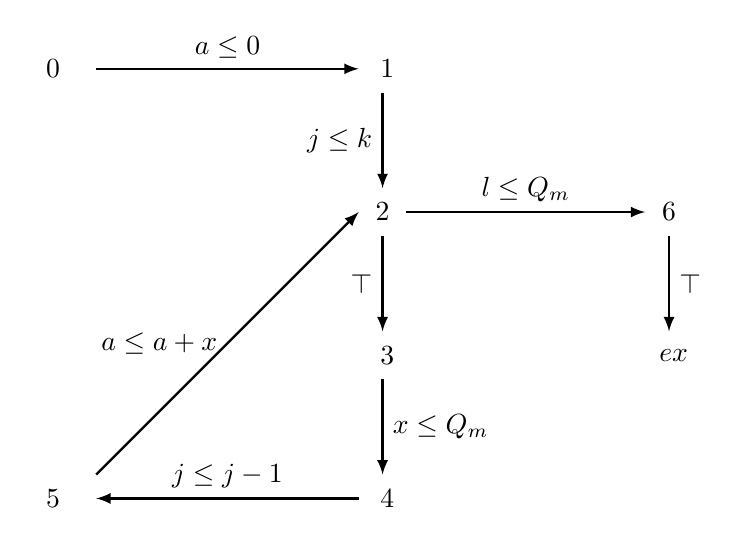
\begin{tikzpicture}[scale=\textwidth/20cm,samples=200]
    \draw[] (-7, 10) circle (0pt) node{{ $0$}};
    \draw[] (0, 10) circle (0pt) node{{ $1$}};
    \draw[] (0, 7) circle (0pt) node{\textbf{$2$}};
    \draw[] (0, 4) circle (0pt) node{{ $3$}};
    \draw[] (0, 1) circle (0pt) node{{ $4$}};
    \draw[] (-7, 1) circle (0pt) node{{ $5$}};
    % Counter Variables
    \draw[] (6, 7) circle (0pt) node {\textbf{$6$}};
    \draw[] (6, 4) circle (0pt) node {{ $ex$}};
    %
    % Control Flow Edges:
    \draw[ thick, -latex] (-6, 10)  -- node [above] {$a \leq 0$}(-0.5, 10);
    \draw[ thick, -latex] (0, 9.5)  -- node [left] {$j \leq k$} (0, 7.5) ;
    \draw[ thick, -latex] (0, 6.5)  -- node [left] {$\top$}  (0, 4.5);
    \draw[ thick, -latex] (0, 3.5)  -- node [right] {$x \leq Q_m$} (0, 1.5) ;
    \draw[ thick, -latex] (-0.5, 1)  -- node [above] {$j \leq j - 1$} (-6, 1) ;
    \draw[ thick, -latex] (-6, 1.5)  -- node [left] {$a \leq a + x$} (-0.5, 7)  ;
    \draw[ thick, -latex] (0.5, 7)  -- node [above] {$l \leq Q_m$}  (5.5, 7);
    \draw[ thick, -latex] (6, 6.5)  -- node [right] {$\top$} (6, 4.5) ;
    \end{tikzpicture}
    \caption{}
      \end{centering}
      \end{subfigure}
      \begin{subfigure}{.35\textwidth}
        \begin{centering}
      %   \todo{abstract-cfg for two round}
      \begin{tikzpicture}[scale=\textwidth/20cm,samples=200]
      \draw[] (-10, 10) circle (0pt) node{{ $0: 1$}};
      \draw[] (0, 10) circle (0pt) node{{ $1: 1$}};
      \draw[] (0, 7) circle (0pt) node{\textbf{$2: k$}};
      \draw[] (0, 4) circle (0pt) node{{ $3: k$}};
      \draw[] (0, 1) circle (0pt) node{{ $4: k$}};
      \draw[] (-10, 1) circle (0pt) node{{ $5: k$}};
      % Counter Variables
      \draw[] (6, 7) circle (0pt) node {\textbf{$6: 1$}};
      \draw[] (6, 4) circle (0pt) node {{ $ex: 1$}};
      %
      % Control Flow Edges:
    \draw[ thick, -latex] (-8, 10)  -- node [above] {$a \leq 0$}(-1.5, 10);
    \draw[ thick, -latex] (0, 9.5)  -- node [left] {$j \leq k$} (0, 7.5) ;
    \draw[ thick, -latex] (0, 6.5)  -- node [left] {$\top$}  (0, 4.5);
    \draw[ thick, -latex] (0, 3.5)  -- node [right] {$x \leq Q_m$} (0, 1.5) ;
    \draw[ thick, -latex] (-1.5, 1)  -- node [above] {$j \leq j - 1$} (-8, 1) ;
    \draw[ thick, -latex] (-8, 1.5)  -- node [left] {$a \leq a + x$} (-1.5, 7)  ;
    \draw[ thick, -latex] (1.5, 7)  -- node [above] {$l \leq Q_m$}  (4.5, 7);
    \draw[ thick, -latex] (6, 6.5)  -- node [right] {$\top$} (6, 4.5) ;
      \end{tikzpicture}
      \caption{}
        \end{centering}
        \end{subfigure}
    %       \begin{subfigure}{.3\textwidth}
    %   \begin{centering}
    %   \begin{tikzpicture}[scale=\textwidth/18cm,samples=200]
    % \draw[] (0, 10) circle (0pt) node
    % {{ $a^0: {}^1_{0}$}};
    % \draw[] (0, 7) circle (0pt) node
    % {\textbf{$x^3: {}^{k}_{1}$}};
    % \draw[] (0, 4) circle (0pt) node
    % {{ $a^5: {}^{k}_{0}$}};
    % \draw[] (0, 1) circle (0pt) node
    % {{ $l^6: {}^{1}_{1}$}};
    % % Counter Variables
    % \draw[] (5, 9) circle (0pt) node {\textbf{$j^2: {}^{1}_{0}$}};
    % \draw[] (5, 6) circle (0pt) node {{ $j^4: {}^{k}_{0}$}};
    % %
    % % Value Dependency Edges:
    % \draw[ ultra thick, -latex, densely dotted,] (0, 1.5)  -- (0, 3.5) ;
    % \draw[ ultra thick, -latex, densely dotted,] (0, 4.5)  -- (0, 6.5) ;
    % \draw[ thick, -latex] (0, 7.5)  -- (0, 9.5) ;
    % \draw[ thick, -Straight Barb] (1.5, 3.5) arc (120:-200:1);
    % \draw[ thick, -Straight Barb] (6.5, 6.5) arc (150:-150:1);
    % \draw[ thick, -latex] (5, 6.5)  -- (5, 8.5) ;
    % % Control Dependency
    % \draw[ thick,-latex] (1.5, 7)  -- (4, 9) ;
    % \draw[ thick,-latex] (1.5, 4)  -- (4, 9) ;
    % \draw[ thick,-latex] (1.5, 7)  -- (4, 6) ;
    % \draw[ thick,-latex] (1.5, 4)  -- (4, 6) ;
    % \end{tikzpicture}
    % \caption{}
    %   \end{centering}
    %   \end{subfigure}
      \vspace{-0.3cm}
      \caption{(a) The same $\kw{towRounds(k)}$ program as Figure~\ref{fig:overview-example}
      (b) The abstract control flow graph for $\kw{towRounds(k)}$  (c) The abstract control flow graph with the reachability bound for $\kw{towRounds(k)}$.}
      \vspace{-0.5cm}
      \label{fig:abscfg_twoRounds}
    \end{figure}
}
\end{example}